\documentclass[a4paper, 11pt]{report}
\usepackage[margin=1cm]{geometry}
\usepackage{booktabs,siunitx}
\usepackage{amsmath, amssymb, amsfonts, float, graphicx, pdfpages, caption}
\usepackage{blindtext}
\renewcommand{\bibname}{References}

\pagenumbering{gobble}

\begin{document}
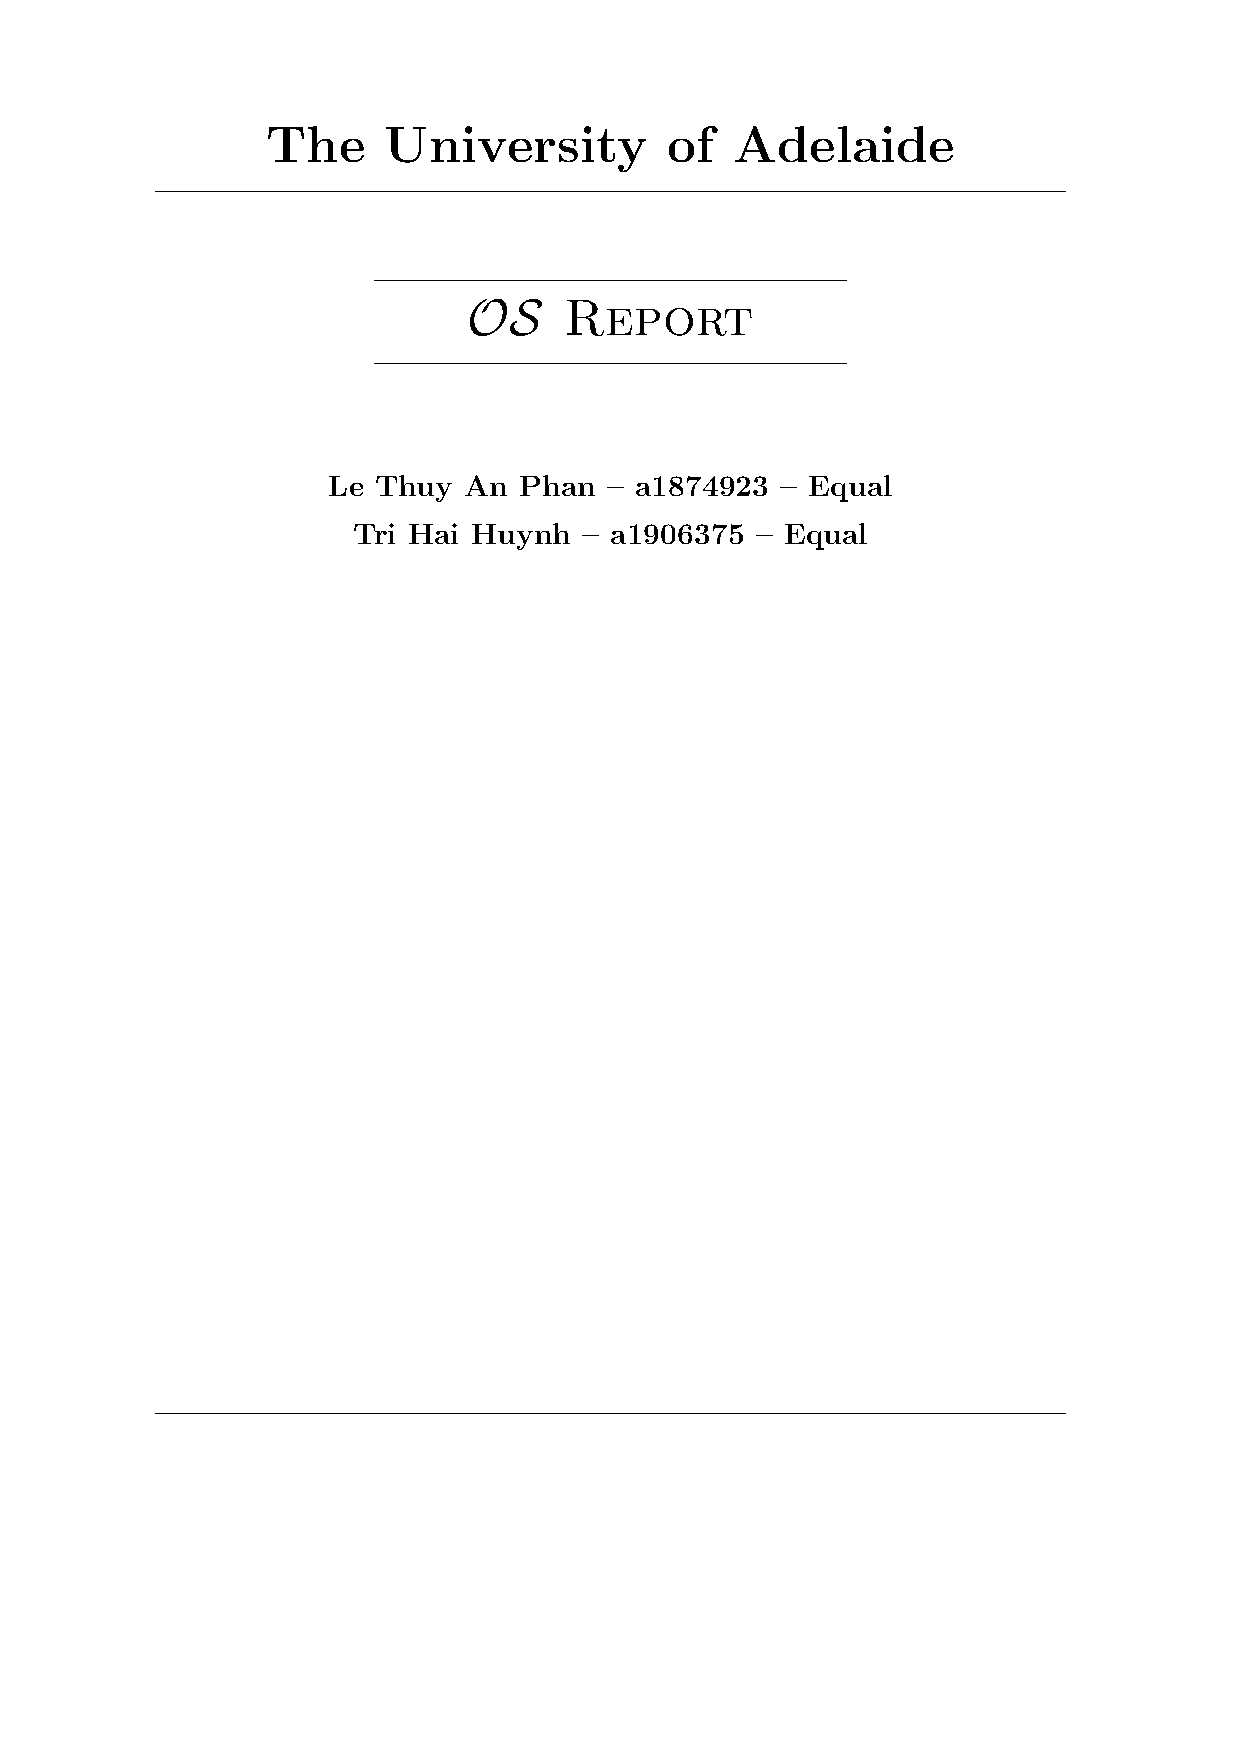
\includepdf[pages={1}, scale = 1]{../bin/page_cover.pdf}
\newpage
\section*{Introduction}
    \quad\quad Efficient management of main memory is a central challenge for operating systems. Virtual memory addresses this by giving programs the illusion of a larger memory than physically available: data not currently in RAM can be stored on secondary storage (disk) and brought into memory on demand. Virtual memory is divided into fixed-size units called \emph{pages}, which are loaded into a limited number of physical page frames in RAM. When a program accesses a page that is not resident in memory, a \emph{page fault} occurs and the operating system must choose which resident page to evict to make room for the requested page.
    The choice of page-replacement policy directly affects the page-fault rate and therefore overall system performance, because disk I/O is orders of magnitude slower than memory access. Inefficient policies produce high fault rates and degrade throughput and responsiveness. In this project we investigate four page-replacement policies implemented in our simulator: \texttt{Rand} (Random), \texttt{LRU} (Least Recently Used), \texttt{Clock} (approximation to LRU), and \texttt{Optimal} (theoretical benchmark).
    The purpose of this report is to evaluate and compare the performance of these algorithms on real-world memory traces. More specifically, we aim to answer the following research questions:
    \begin{enumerate}
        \item How does the number of available page frames affect the page-fault rate for each algorithm in a set of population of types of memory trace?
        \item Which algorithm performs best when the number of available frames is insufficient (i.e., extreme thrashing)?
        \item Do results vary significantly across different memory access patterns (different traces)?
    \end{enumerate}
\section*{Methodology}
\label{sec:methodology}

This section describes the simulation environment, and the experimental design used to collect performance data.

\subsection*{Simulator and environment setup}
\label{ssec:simulator}
We developed a simulator in Python that models a single-level page table and evaluates page-replacement policies on real trace inputs. To ensure fair comparison the simulator used the following fixed parameters:
\begin{itemize}
  \item \textbf{Page and frame size:} 4~KB.
  \item \textbf{Trace inputs:} Each run processes one memory trace containing 1\,000\,000 memory accesses. The traces used in this report are \texttt{bzip}, \texttt{gcc}, \texttt{sixpack} and \texttt{swim}.
  \item \textbf{Primary metric:} \emph{Page-fault rate}$\;=\; \frac{\text{Total Page Faults}}{\text{Total Memory Accesses}}$
  . Total disk reads and writes are also recorded, but the page-fault rate is used as the core metric for visualisation and analysis because it directly reflects the frequency of expensive disk I/O events.
\end{itemize}

\subsection*{Experimental design}
\begin{itemize}
    \item \textbf{Low Frame Size:} evaluate robustness and thrashing behaviour when frames are scarce.
    \item \textbf{Medium Frame Size:} identify where the largest marginal improvement occurs and estimate the program's working-set size.
    \item \textbf{High Frame Size:} show convergence of page-fault rates as additional frames yield diminishing returns.
    \item \textbf{Statistical Inference:} to determine if the observed differences between the algorithms were statistically significant, a Matched Pair $t$-test was employed, however with the assumption that the mean differences between the algorithms are normally distributed.
    \item \textbf{Mean Table:} a mean table of different segments of a specific trace of each algorithm to numerically describe the overall performance of each algorithm.
    \item \textbf{Mean Table:} each result of a trace file is plotted by Matplotlib with x-axis as frame size and y-axis as page fault rate in a line graph.
\end{itemize}
\newpage
\section*{GCC Trace}
    \begin{table}[ht]
        \centering
        \label{tab:means_plain}
        \begin{tabular}{l c c c c}
            \toprule
            Segment & LRU & RAND & CLOCK & OPTIMAL \\
            \hline
            1--200  & 0.0644 & 0.0806 & 0.0678 & 0.0431 \\
            1--10   & 0.2744 & 0.3250 & 0.2957 & 0.2228 \\
            10--75  & 0.0805 & 0.1023 & 0.0838 & 0.0534 \\
            75--200 & 0.0399 & 0.0507 & 0.0420 & 0.0239 \\
            \hline
            Mean    & 0.1148 & 0.1397 & 0.1223 & 0.0858 \\
            \bottomrule
        \end{tabular}
        \caption{Mean fault rates by segment and algorithm}
    \end{table}
    \begin{quote}
        OPTIMAL consistently outperforms others with the overall fault rate mean of 0.0858, while RAND is the worst with fault rate of 0.1397. LRU and CLOCK are close, with LRU slightly better in 
        thrashing scenario, low frames (1-10: 0.2744 $<$ 0.2957), suggesting LRU performs better than CLOCK's approximation of LRU in high-fault scenarios. 
        The overall performance is on average $+0.02\rightarrow+0.05$ fault rate from the OPTIMAL. 
    \end{quote}
    \begin{table}[ht]
        \centering
        \label{tab:pairwise}
        \begin{tabular}{l
                        S[table-format=1.0]
                        S[table-format=-2.4]
                        S[table-format=1.0]
                        S[table-format=1.4]
                        S[table-format=1.4]
                        S[table-format=-1.4]
                        S[table-format=1.4]}
            \toprule
            {Comparison} & {n} & {t\_stat} & {df} & {p\_value} & {mean\_diff} & {diff\_low} & {diff\_high} \\
            \midrule
            \texttt{lru\_vs\_rand}     & 4 & -2.8009 & 3 & 0.0678 & -0.0249 & -0.0531 & 0.0034 \\
            \texttt{lru\_vs\_clock}    & 4 & -1.6355 & 3 & 0.2005 & -0.0075 & -0.0222 & 0.0071 \\
            \texttt{lru\_vs\_optimal}  & 4 &  3.6863 & 3 & \boxed{0.0346} &  0.0290 &  0.0040 & 0.0540 \\
            \texttt{rand\_vs\_clock}   & 4 &  3.8768 & 3 & \boxed{0.0304} &  0.0173 &  0.0031 & 0.0315 \\
            \texttt{rand\_vs\_optimal} & 4 &  3.2176 & 3 & \boxed{0.0487} &  0.0538 &  0.0006 & 0.1071 \\
            \texttt{clock\_vs\_optimal}& 4 &  2.9497 & 3 & 0.0600 &  0.0365 & -0.0029 & 0.0759 \\
            \bottomrule
        \end{tabular}
        \caption{Pairwise comparison statistics\cite{psu_paired}}
    \end{table}
    \begin{quote}
        Based on the samples, I am 95\% confident that the following differences are statistically significant at the $\text{p-value}<0.05$\cite{psu_paired}: 
        \begin{itemize}
            \item Mean fault rate difference (LRU $-$ OPTIMAL) is between $[0.0040,\;0.0540]$
            \item Mean fault rate difference (RAND $-$ CLOCK) is between $[0.0031,\;0.0315]$ 
            \item Mean fault rate difference (RAND $-$ OPTIMAL) is between $[0.0006,\;0.1071]$
        \end{itemize}
            Thus, at the 95\% confidence level we conclude that LRU performs significantly worse than OPTIMAL, and RAND performs significantly worse than 
            CLOCK and OPTIMAL on the GCC memory trace sample.
    \end{quote}
    \begin{flushright}
        \vspace{0.5cm}
        \begin{minipage}[t]{0.5\linewidth}
            \begin{quote}
                Across all segments, fault rates display exponential decay as frame size increases. RAND has the highest rates, 
                visually separating from others, supporting its significant inferiority to CLOCK and OPTIMAL. LRU and CLOCK lines stay closely with each other in all 
                segments, explaining the high p\_value $\approx 0.2005$. In extreme thrashing (1-10), LRU edges slightly lower, but all go to convergence by 75-200 
                aligns with the overall performance of the Table 1. Overall, the visuals reinforce the theoretical sample trends of GCC memory trace.
                Additionally, the data here has a strong evidence of supporting each other.
            \end{quote}
        \end{minipage}
    \end{flushright}
    \begin{figure}[H]
        \includepdf[pages={1}, scale = 0.5, offset=-100 -270]{../../graph/gcc_ranges_1-4096_fs-pfr_line_slices_0-199_0-9_9-74_74-199.pdf}
    \end{figure}

\newpage
\section*{Bzip Trace}
    % -----------------------------
    % Table 1: Segment means
    % -----------------------------
    \begin{table}[ht]
        \centering
        \label{tab:segment_means}
        \begin{tabular}{l
                        S[table-format=1.4]
                        S[table-format=1.4]
                        S[table-format=1.4]
                        S[table-format=1.4]}
            \toprule
            Segment & {LRU} & {RAND} & {CLOCK} & {OPTIMAL} \\
            \midrule
            1--200  & 0.0072 & 0.0089 & 0.0083 & 0.0063 \\
            1--10   & 0.1218 & 0.1503 & 0.1429 & 0.1123 \\
            10--75  & 0.0022 & 0.0028 & 0.0025 & 0.0014 \\
            75--200 & 0.0007 & 0.0009 & 0.0008 & 0.0005 \\
            \hline
            Mean    & 0.0330 & 0.0407 & 0.0386 & 0.0301\\
            \bottomrule
        \end{tabular}
        \caption{Mean fault rates by segment and algorithm}
    \end{table}
    \begin{quote}
        OPTIMAL has the lowest overall mean fault rate (0.0301) while RAND is highest (0.0407). CLOCK and RAND are very close in every segment, and the mean gap 
        $0.0056_{clock-lru} > 0.0021_{rand-clock}$, indicating CLOCK is closer to RAND than to LRU despite being an approximate of LRU. 
        During the working-set frame count (10-75) the difference starts to normalise. At higher frame counts (75-200), LRU approaches OPTIMAL, while CLOCK remains 
        to be closer to RAND than LRU.
    \end{quote}

    % -----------------------------
    % Table 2: Pairwise comparisons
    % -----------------------------
    \begin{table}[ht]
        \centering
        \label{tab:pairwise2}
        \begin{tabular}{l
                        S[table-format=1.0]
                        S[table-format=-1.4]
                        S[table-format=1.0]
                        S[table-format=1.4]
                        S[table-format=-1.4]
                        S[table-format=-1.4]
                        S[table-format=1.4]}
            \toprule
            {Comparison} & {n} & {t\_stat} & {df} & {p\_value} & {diff\_low} & {diff\_high} \\
            \midrule
            \texttt{lru\_vs\_rand}     & 4 & -1.1193 & 3 & 0.3445 & -0.0298 & 0.0143 \\
            \texttt{lru\_vs\_clock}    & 4 & -1.0961 & 3 & \boxed{0.3531} & -0.0221 & 0.0108 \\
            \texttt{lru\_vs\_optimal}  & 4 &  1.2826 & 3 & 0.2898 & -0.0042 & 0.0099 \\
            \texttt{rand\_vs\_clock}   & 4 &  1.1867 & 3 & 0.3208 & -0.0035 & 0.0077 \\
            \texttt{rand\_vs\_optimal} & 4 &  1.1592 & 3 & 0.3303 & -0.0185 & 0.0397 \\
            \texttt{clock\_vs\_optimal}& 4 &  1.1526 & 3 & 0.3326 & -0.0150 & 0.0320 \\
            \bottomrule
        \end{tabular}
        \caption{Pairwise comparison statistics\cite{psu_paired}}
    \end{table}    
    \begin{quote}
        Based on the samples, at 95\% confidence level, none of the pairwise differences are statistically significant, all $\text{p-value}>0.05$\cite{psu_paired}.\\
        Thus, we cannot conclude any algorithm differs significantly from another on the Bzip memory trace sample. However, the statistics show that the 
        weakest difference is between LRU-CLOCK which contradicts with the mean table 3 that shows otherwise.
    \end{quote}
    \begin{flushright}
        \vspace{0.5cm}
        \begin{minipage}[t]{0.5\linewidth}
            \begin{quote}
                Across all segments, fault rates display exponential decay as frame size increases. In the frame size of (20-200), RAND and OPTIMAL serve as
                the upper and lower bounds. However, the first segment (1-200) display a local lump from CLOCK,
                can be explained by CLOCK temporarily degenerate to FIFO\cite{cornelluni}. As we also know that FIFO will suffer from the Belady's Anomaly. So,
                CLOCK exhibit the anomaly, in that when increasing frame size the fault rate goes 
                up\cite{ostep2018}. Overall, the visuals reinforce theoretical assumption of the table 3 as CLOCK-RAND go closely across. 
                While, after the anomaly, CLOCK and LRU consistently approache OPTIMAL at larger frame size, which supports inference from table 4.
            \end{quote}
        \end{minipage}
    \end{flushright}
    \begin{figure}[H]
        \includepdf[pages={1}, scale = 0.5, offset=-100 -230]{../../graph/bzip_ranges_1-4096_fs-pfr_line_slices_0-199_0-9_9-74_74-199.pdf}
    \end{figure}
\newpage
\section*{Swim Trace}
% -----------------------------
% Table 1: Segment means
% -----------------------------
    \begin{table}[ht]
        \centering
        \label{tab:segment_means_3}
        \begin{tabular}{l
                        S[table-format=1.4]
                        S[table-format=1.4]
                        S[table-format=1.4]
                        S[table-format=1.4]}
            \toprule
            Segment & {LRU} & {RAND} & {CLOCK} & {OPTIMAL} \\
            \midrule
            1--200  & 0.0454 & 0.0594 & 0.0490 & 0.0288 \\
            1--10   & 0.3723 & 0.4233 & 0.3935 & 0.2843 \\
            10--75  & 0.0615 & 0.0859 & 0.0666 & 0.0336 \\
            75--200 & 0.0125 & 0.0182 & 0.0138 & 0.0068 \\
            \hline
            Mean    & 0.1229 & 0.1467 & 0.1307 & 0.0884 \\
            \bottomrule
        \end{tabular}
        \caption{Mean fault rates by segment and algorithm}
    \end{table}
    \begin{quote}
        OPTIMAL consistently outperforms others with the overall mean 0.0884, while RAND is worst (0.1467). LRU and CLOCK are close, with LRU slightly better in 
        thrashing scenario, low frames (1-10: 0.3723 $<$ 0.3935), suggesting LRU performs better than CLOCK's approximation of LRU in high-fault scenarios. The
        overall performance is on average $+0.04\rightarrow+0.06$ fault rate from the OPTIMAL.
    \end{quote}
    % -----------------------------
% Table 2: Pairwise comparisons
% -----------------------------
    \begin{table}[ht]
        \centering
        \label{tab:pairwise_3}
        \begin{tabular}{l
                        S[table-format=1.0]
                        S[table-format=-2.4]
                        S[table-format=1.0]
                        S[table-format=1.4]
                        S[table-format=-1.4]
                        S[table-format=-1.4]
                        S[table-format=1.4]}
            \toprule
            {Comparison} & {n} & {t\_stat} & {df} & {p\_value} & {mean\_diff} & {diff\_low} & {diff\_high} \\
            \midrule
            \texttt{lru\_vs\_rand}     & 4 & -2.4141 & 3 & \boxed{0.0947} & -0.0238 & -0.0551 & 0.0076 \\
            \texttt{lru\_vs\_clock}    & 4 & -1.7201 & 3 & \boxed{0.1839} & -0.0078 & -0.0222 & 0.0066 \\
            \texttt{lru\_vs\_optimal}  & 4 &  1.8794 & 3 & 0.1568 &  0.0346 & -0.0240 & 0.0931 \\
            \texttt{rand\_vs\_clock}   & 4 &  2.8877 & 3 & \boxed{0.0631} &  0.0160 & -0.0016 & 0.0336 \\
            \texttt{rand\_vs\_optimal} & 4 &  2.0712 & 3 & 0.1301 &  0.0583 & -0.0313 & 0.1479 \\
            \texttt{clock\_vs\_optimal}& 4 &  1.8488 & 3 & 0.1616 &  0.0424 & -0.0305 & 0.1152 \\
            \bottomrule
        \end{tabular}
        \caption{Pairwise comparison statistics\cite{psu_paired}}
    \end{table}
    \begin{quote}
        Based on the samples, at 95\% confidence level, none of the pairwise differences are statistically significant, all $\text{p-value}>0.05$\cite{psu_paired}.\\
        Thus, we cannot conclude any algorithm differs significantly from another on the Swim memory trace sample.
    \end{quote}
    \begin{flushright}
        \vspace{0.5cm}
        \begin{minipage}[t]{0.5\linewidth}
            \begin{quote}
                Across all segments, fault rates display exponential decay as frame size increases. RAND and OPTIMAL serve as a clear uppper and lower bounds.
                The relationship between RAND-LRU-CLOCK in the visuals support the inference from Table 6, as the p-value of LRU-CLOCK is highest therefore 
                go together closely while having insignificant difference with RAND. In the working set frame size (10-75), with the current evidence and visuals
                CLOCK has a small lump this shows that CLOCK has almost degenerated to FIFO\cite{cornelluni}. Overall, the visuals reinforce the theoretical 
                sample trends from Table 5, which LRU-CLOCK on average go closely together and RAND is the worst on average, and Table 6 of Swim trace.
                Additionally, the data here has a strong evidence of supporting each other.
            \end{quote}
        \end{minipage}
    \end{flushright}
    \begin{figure}[H]
        \includepdf[pages={1}, scale = 0.5, offset=-100 -220]{../../graph/swim_ranges_1-4096_fs-pfr_line_slices_0-199_0-9_9-74_74-199.pdf}
    \end{figure}
\newpage
\section*{Sixpack Trace}
% -----------------------------
% Table 1: Segment means
% -----------------------------
    \begin{table}[ht]
        \centering
        \label{tab:segment_means_latest}
        \begin{tabular}{l
                        S[table-format=1.4]
                        S[table-format=1.4]
                        S[table-format=1.4]
                        S[table-format=1.4]}
            \toprule
            Segment & {LRU} & {RAND} & {CLOCK} & {OPTIMAL} \\
            \midrule
            1--200  & 0.0488 & 0.0630 & 0.0523 & 0.0317 \\
            1--10   & 0.3054 & 0.3595 & 0.3315 & 0.2401 \\
            10--75  & 0.0656 & 0.0848 & 0.0688 & 0.0392 \\
            75--200 & 0.0204 & 0.0290 & 0.0222 & 0.0116 \\
            \hline
            Mean    & 0.1101 & 0.1341 & 0.1187 & 0.0807 \\
            \bottomrule
        \end{tabular}
        \caption{Mean fault rates by segment and algorithm}
    \end{table}
    \begin{quote}
        OPTIMAL consistently outperforms others with the overall fault rate mean of 0.0807, while RAND is worst with fault rate at 0.1341. LRU and CLOCK are close, with LRU slightly better in 
        thrashing scenario, low frames (1-10: 0.3054 $<$ 0.3315), suggesting LRU performs better than CLOCK's approximation of LRU in high-fault scenarios. The
        overall performance is on average $+0.03\rightarrow+0.05$ fault rate from the OPTIMAL.
    \end{quote}
    % -----------------------------
% Table 2: Pairwise comparisons
% -----------------------------
    \begin{table}[ht]
        \centering
        \label{tab:pairwise_latest}
        \begin{tabular}{l
                        S[table-format=1.0]
                        S[table-format=-2.4]
                        S[table-format=1.0]
                        S[table-format=1.4]
                        S[table-format=-1.4]
                        S[table-format=-1.4]
                        S[table-format=1.4]}
            \toprule
            {Comparison} & {n} & {t\_stat} & {df} & {p\_value} & {mean\_diff} & {diff\_low} & {diff\_high} \\
            \midrule
            \texttt{lru\_vs\_rand}     & 4 & -2.3425 & 3 & 0.1010 & -0.0240 & -0.0567 & 0.0086 \\
            \texttt{lru\_vs\_clock}    & 4 & -1.4841 & 3 & \boxed{0.2344} & -0.0087 & -0.0272 & 0.0099 \\
            \texttt{lru\_vs\_optimal}  & 4 &  2.3530 & 3 & 0.1000 &  0.0294 & -0.0104 & 0.0692 \\
            \texttt{rand\_vs\_clock}   & 4 &  3.3342 & 3 & \boxed{0.0446} &  0.0154 &  0.0007 & 0.0301 \\
            \texttt{rand\_vs\_optimal} & 4 &  2.3502 & 3 & 0.1003 &  0.0534 & -0.0189 & 0.1258 \\
            \texttt{clock\_vs\_optimal}& 4 &  2.0905 & 3 & 0.1277 &  0.0380 & -0.0199 & 0.0960 \\
            \bottomrule
        \end{tabular}
        \caption{Pairwise comparison statistics\cite{psu_paired}}
    \end{table}
    \begin{quote}
        Based on the samples, I am 95\% confident that the following differences are statistically significant at the $\text{p-value}<0.05$\cite{psu_paired}: 
        \begin{itemize}
            \item Mean fault rate difference (RAND $-$ CLOCK) is between $[0.0007,\;0.0301]$
        \end{itemize}
            Thus, at the 95\% confidence level we conclude that RAND performs significantly worse than CLOCK on the Sixpack memory trace.
    \end{quote}
    \begin{flushright}
        \vspace{0.5cm}
        \begin{minipage}[t]{0.5\linewidth}
            \begin{quote}
                Across all segments, fault rates display exponential decay as frame size increases. RAND and OPTIMAL serve as the upper and lower bounds 
                . LRU and CLOCK lines stay closely with each other in all 
                segments, explaining the high p\_value $\approx 0.2344$ in Table 8. In extreme thrashing (1-10), LRU edges slightly lower, but all go to convergence by 75-200 
                aligns with the overall performance of the Table 7. Overall, the visuals reinforce the theoretical sample trends of Sixpack memory trace.
                Additionally, the data here has a strong evidence of supporting each other.
            \end{quote}
        \end{minipage}
    \end{flushright}
    \begin{figure}[H]
        \includepdf[pages={1}, scale = 0.5, offset=-100 -250]{../../graph/sixpack_ranges_1-4096_fs-pfr_line_slices_0-199_0-9_9-74_74-199.pdf}
    \end{figure}
\newpage
\section*{Conclusion}
    \begin{quote}
        \quad\quad In conclusion, the evidence strongly supports that the number of available page frames affect the page-fault rate for each algorithm across different types of memory traces. For example, when frame size increase, page-fault rate usually drop, but it depend on the algorithm, such as CLOCK might degenerate to FIFO which would produce more faults in sequential traces, while LRU behaves better. There exists a working set size that is the optimal amount of frames which yield a good page fault rate. Regarding of which algorithm performs best in extreme thrashing, the evidence shows LRU is consistent through memory traces under such condition. Finally, the evidence supports that the result does not have big variation between traces, by that LRU stays as a top performer, and CLOCK often approximates LRU correctly, even in phased traces like bzip where bump happen but not too disruptive overall. This suggests algorithms are robust in general. 
    \end{quote}
\bibliographystyle{plain}
\bibliography{ref}
\end{document}